\section{二叉树、资产组合复制和套利}
\subsection{衍生产品定价的三种方法}
本节无习题
\subsection{博弈论方法}
\begin{enumerate}
    \item \sol \textcolor{blue}{本题中的10美元应为110美元.}\\
    法一(博弈论方法):
    \begin{align*}
        a & = \frac{U-D}{S_u-S_d} = \frac{10-0}{130-100}=\frac{1}{3},\\
        V_0 & = aS_0 + (U-aS_u)\e^{-r\tau}\\
        & = \frac{1}{3} \times 110 + \left(10-\frac{1}{3} \times 130\right)\e^{-0.04}\\
        & = 4.62 \text{ (美元) 或 } 4.64 \text{ (美元)}
    \end{align*}
    若$\e^{-0.04}$取近似值$\displaystyle\frac{1}{1.04}$,结果为4.62美元;若不近似,直接计算,结果为4.64美元.\\
    法二(期望价值定价方法):\\
    先计算风险中性概率:\[q = \frac{\e^{r\tau}S_0 - S_d}{S_u - S_d} = \frac{\e^{0.04} \times 110 - 100}{130-100} = 0.48 \text{ 或 } 0.4830\]
    其中,0.48是取近似结果,0.4830是直接计算结果.
    \begin{align*}
        V_0 & = \e^{-r\tau}[qU+(1-q)D]\\
        & = \e^{-0.04}(10q+0)\\
        & = 4.62 \text{ (美元) 或 } 4.64 \text{ (美元)}
    \end{align*}
    其中,4.62是取近似结果,4.64是直接计算结果.\\
    法三(概率方法):
    \[E(\Pi_1) = 130p + 100(1-p) = 30p+100 = 110 \times 1.04 = 114.4 \Rightarrow p = 0.48\]
    则
    \[E(C) = 0.48 \times 10 + 0.52 \times 0 = 4.8 \Rightarrow V_0 = \frac{E(C)}{1.04} = 4.62\]
    所以,价格为4.62美元.
    \item \sol\\
    法一(博弈论方法):\\
    由题意:$U=S_u-X=130-100=30,D=0$,则
    \begin{align*}
        a & = \frac{U-D}{S_u-S_d} = \frac{30-0}{130-100}=1,\\
        V_0 & = aS_0 + (U-aS_u)\e^{-r\tau}\\
        & = 1 \times 110 + \left(30-1 \times 130\right)\e^{-0.04}\\
        & = 13.85 \text{ (美元) 或 } 13.92 \text{ (美元)}
    \end{align*}
    若$\e^{-0.04}$取近似值$\displaystyle\frac{1}{1.04}$,结果为13.85美元;若不近似,直接计算,结果为13.92美元.\\
    法二(期望价值定价方法):\\
    先计算风险中性概率:\[q = \frac{\e^{r\tau}S_0 - S_d}{S_u - S_d} = \frac{\e^{0.04} \times 110 - 100}{130-100} = 0.48 \text{ 或 } 0.4830\]
    其中,0.48是取近似结果,0.4830是直接计算结果.
    \begin{align*}
        V_0 & = \e^{-r\tau}[qU+(1-q)D]\\
        & = \e^{-0.04}(30q+0)\\
        & = 13.85 \text{ (美元) 或 } 13.92 \text{ (美元)}
    \end{align*}
    其中,13.85是取近似结果,13.92是直接计算结果.\\
    法三(概率方法):
    \[E(\Pi_1) = 130p + 100(1-p) = 30p+100 = 110 \times 1.04 = 114.4 \Rightarrow p = 0.48\]
    则
    \[E(C) = 0.48 \times 30 + 0.52 \times 0 = 14.4 \Rightarrow V_0 = \frac{E(C)}{1.04} = 13.85\]
    所以,价格为13.85美元.
    \item \sol\\
    法一(博弈论方法):
    \begin{align*}
        a & = \frac{U-D}{S_u-S_d} = \frac{0-5}{130-90}=-\frac{1}{8},\\
        V_0 & = aS_0 + (U-aS_u)\e^{-r\tau}\\
        & = -\frac{1}{8} \times 100 + \left(0 +\frac{1}{8} \times 130\right)\e^{-0.05}\\
        & = 2.96
    \end{align*}
    所以,结果为2.96美元.\\
    法二(期望价值定价方法):\\
    先计算风险中性概率:\[q = \frac{\e^{r\tau}S_0 - S_d}{S_u - S_d} = \frac{\e^{0.05} \times 100 - 90}{130-90} = 0.3782\]
    \begin{align*}
        V_0 & = \e^{-r\tau}[qU+(1-q)D]\\
        & = \e^{-0.05}(0q+5(1-q))\\
        & = 2.96
    \end{align*}
    所以,结果为2.96美元.\\
    法三(概率方法):
    \[E(\Pi_1) = 130p + 90(1-p) = 40p+90 = 100 \times 1.05 = 105 \Rightarrow p = 0.375\]
    则
    \[E(C) = 0.375 \times 0 + 0.625 \times 5 = 3.125 \Rightarrow V_0 = \frac{E(C)}{1.05} = 2.99\]
    所以,价格为2.99美元.
    \item \sol\\
    法一(博弈论方法):\\
    由题意:$U=0,D=X-S_d=10$,则
    \begin{align*}
        a & = \frac{U-D}{S_u-S_d} = \frac{0-10}{75-50}=-\frac{2}{5},\\
        V_0 & = aS_0 + (U-aS_u)\e^{-r\tau}\\
        & = -\frac{2}{5} \times 60 + \left(0+\frac{2}{5} \times 75\right)\e^{-0.05}\\
        & = 4.54
    \end{align*}
    所以,结果为4.54美元.\\
    法二(期望价值定价方法):\\
    先计算风险中性概率:\[q = \frac{\e^{r\tau}S_0 - S_d}{S_u - S_d} = \frac{\e^{0.05} \times 60 - 50}{75-50} = 0.5231\]
    \begin{align*}
        V_0 & = \e^{-r\tau}[qU+(1-q)D]\\
        & = \e^{-0.05}(0q+10(1-q))\\
        & = 4.54
    \end{align*}
    所以,结果为4.54美元.\\
    法三(概率方法):
    \[E(\Pi_1) = 75p + 50(1-p) = 25p+50 = 60 \times 1.05 = 63 \Rightarrow p = 0.52\]
    则
    \[E(C) = 0.52 \times 0 + 0.48 \times 10 = 4.8 \Rightarrow V_0 = \frac{E(C)}{1.05} = 4.57\]
    所以,价格为4.57美元.
\end{enumerate}
\subsection{资产组合复制}
本节无习题
\subsection{概率方法}
\begin{enumerate}
    \item \sol\\
    法一(博弈论方法):
    \begin{center}
        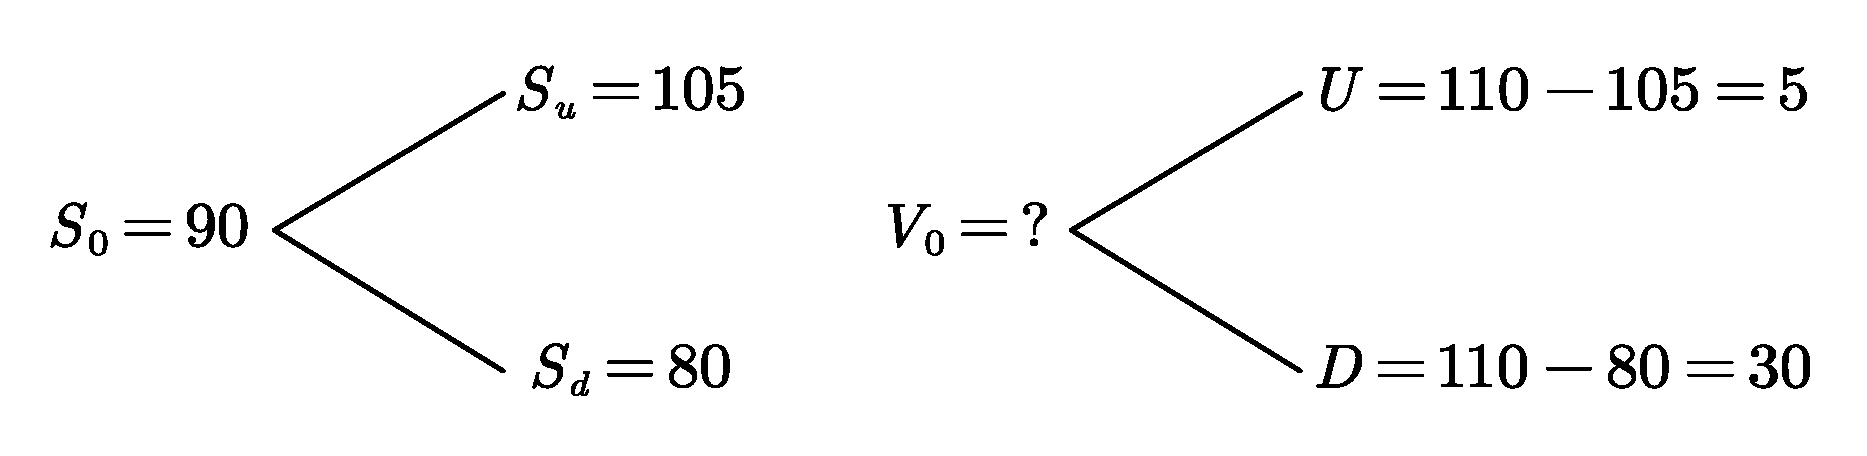
\includegraphics[scale=0.35]{CH2-4-1.pdf}
    \end{center}
    我们通过买入1股期权和卖出$a$股股票构造资产组合. 资产组合的初始价值是:
    \[\Pi_0=V_0-aS_0\]
    我们可以选择$a$的值使得资产组合的价值与股票的最终状态无关.
    \begin{align*}
        &\text{上升时:}\Pi_u = U-aS_u\\
        &\text{下降时:}\Pi_d = D-aS_d
    \end{align*}
    如果令:\[U-aS_u=D-aS_d\]
    那么,我们可以选择\[a = \frac{U-D}{S_u-S_d} = \frac{5-30}{105-80}=-1\]
    我们把$a$引入计算:
    \begin{align*}
        &\text{资产组合的初始成本} = V_0-aS_0\\
        &\text{资产组合的最终价值} = U-aS_u
    \end{align*}
    因为该资产组合投资没有风险,则有:
    \[V_0-aS_0=\e^{-r\tau}(U-aS_u) \Rightarrow V_0 = aS_0 + (U-aS_u)\e^{-r\tau}\]
    代入数值,若$\e^{-0.04}$取近似值$\displaystyle\frac{1}{1.04}$,结果为15.77美元;若不近似,直接计算,结果为15.69美元.\\
    法二(期望价值定价方法):\\
    先计算风险中性概率:\[q = \frac{\e^{r\tau}S_0 - S_d}{S_u - S_d} = \frac{\e^{0.04} \times 90 - 80}{105-80} = 0.544 \text{ 或 } 0.5469\]
    其中,0.544是取近似结果,0.5469是直接计算结果.
    \begin{align*}
        V_0 & = \e^{-r\tau}[qU+(1-q)D]\\
        & = \e^{-0.04}[5q+30(1-q)]\\
        & = 15.77 \text{ (美元) 或 } 15.69 \text{ (美元)}
    \end{align*}
    其中,15.77是取近似结果,15.69是直接计算结果.\\
    法三(概率方法):
    \[E(\Pi_1) = 105p + 80(1-p) = 25p+80 = 90 \times 1.04 = 93.6 \Rightarrow p = 0.544\]
    则
    \[E(C) = 0.544 \times 5 + 0.456 \times 30 = 16.4 \Rightarrow V_0 = \frac{E(C)}{1.04} = 15.77\]
    所以,价格为15.77美元.
    \item \sol\\
    法一(博弈论方法):\\
    由题意:$U=0,D=X-S_d=8$,则
    \begin{align*}
        a & = \frac{U-D}{S_u-S_d} = \frac{0-8}{122-102}=-\frac{2}{5},\\
        V_0 & = aS_0 + (U-aS_u)\e^{-r\tau}\\
        & = -\frac{2}{5} \times 110 + \left(0+\frac{2}{5} \times 122\right)\e^{-0.04}\\
        & = 2.89
    \end{align*}
    所以,结果为2.89美元.\\
    法二(期望价值定价方法):\\
    先计算风险中性概率:\[q = \frac{\e^{r\tau}S_0 - S_d}{S_u - S_d} = \frac{\e^{0.04} \times 110 - 102}{122-102} = 0.6245\]
    \begin{align*}
        V_0 & = \e^{-r\tau}[qU+(1-q)D]\\
        & = \e^{-0.04}(0q+8(1-q))\\
        & = 4.54
    \end{align*}
    所以,结果为2.89美元.\\
    法三(概率方法):
    \[E(\Pi_1) = 122p + 102(1-p) = 20p+102 = 110 \times 1.04 = 114.4 \Rightarrow p = 0.62\]
    则
    \[E(C) = 0.62 \times 0 + 0.38 \times 8 = 3.04 \Rightarrow V_0 = \frac{E(C)}{1.04} = 2.92\]
    所以,价格为2.92美元.
    \item \pro\\
    即证:
    \[aS_0 + (U-aS_u)\e^{-r\tau} - \e^{-r\tau}[qU+(1-q)D] = 0\]
    所以,
    \begin{align*}
        & aS_0 + (U-aS_u)\e^{-r\tau} - \e^{-r\tau}[qU+(1-q)D]\\
        = & \frac{U-D}{S_u-S_d}S_0 + \e^{-r\tau}\left(U-\frac{U-D}{S_u-S_d}S_u\right) - \e^{-r\tau}\left(\frac{\e^{r\tau}S_0 - S_d}{S_u - S_d} U + \frac{S_u - \e^{r\tau}S_0}{S_u - S_d}D\right)\\
        = & \e^{-r\tau} \left[\frac{\e^{r\tau}S_0U-\e^{r\tau}S_0D}{S_u - S_d} + U-\frac{U-D}{S_u-S_d}S_u + \frac{\e^{r\tau}S_0 - S_d}{S_u - S_d} U + \frac{S_u - \e^{r\tau}S_0}{S_u - S_d}D\right] = 0
    \end{align*}
    \item \omitted
    \item \pro\\
    因为$U = S_u - X,D = S_d-X$,则
    \begin{align*}
        V_0 & = \e^{-r\tau}[qU+(1-q)D] = \e^{-r\tau}\left(\frac{\e^{r\tau}S_0 - S_d}{S_u - S_d} U + \frac{S_u - \e^{r\tau}S_0}{S_u - S_d}D\right)\\
        & = \e^{-r\tau}\left(\frac{\e^{r\tau}US_0 - US_d + DS_u - \e^{r\tau}DS_0}{U-D}\right)\\
        & = \e^{-r\tau}\left[\frac{\e^{r\tau}US_0 - U(D+X) + D(U+X) - \e^{r\tau}DS_0}{U-D}\right]\\
        & = \e^{-r\tau}\left[\frac{\e^{r\tau}S_0(U-D) - X(U-D)}{U-D}\right]\\
        & = \e^{-r\tau}(\e^{r\tau}S_0 - X)\\
        & = S_0 - \e^{-r\tau}X
    \end{align*}
    \item \sol
    \begin{enumerate}[label=(\alph*)]
        \item 先计算风险中性概率:\[q = \frac{\e^{r\tau}S_0 - S_d}{S_u - S_d} = \frac{\e^{0.04} \times 100 - 90}{115-90} = 0.5632\]
        \begin{align*}
            V_0 & = \e^{-r\tau}[qU+(1-q)D]\\
            & = \e^{-0.04}(0q+5(1-q))\\
            & = 2.10
        \end{align*}
        所以,结果为2.10美元.
        \item 先计算风险中性概率:\[q = \frac{\e^{r\tau}S_0 - S_d}{S_u - S_d} = \frac{\e^{0.04} \times 100 - 90}{115-90} = 0.5632\]
        \begin{align*}
            V_0 & = \e^{-r\tau}[qU+(1-q)D]\\
            & = \e^{-0.04}(0q+15(1-q))\\
            & = 6.20
        \end{align*}
        所以,结果为6.20美元.\\
        解释:由于$U=0$,$D_b = 3D_a$,所以,结果为3倍
    \end{enumerate}
\end{enumerate}
\subsection{风险}
\begin{enumerate}
    \item \sol \textcolor{blue}{本题中的$r=0.55$应为$r=0.05$.}
    \begin{enumerate}[label=(\alph*)]
        \item 由题意:$U=S_u-X=60-55=5,D=0$,则
        \begin{align*}
            a & = \frac{U-D}{S_u-S_d} = \frac{5-0}{60-40}=\frac{1}{4},\\
            V_0 & = aS_0 + (U-aS_u)\e^{-r\tau}\\
            & = \frac{1}{4} \times 50 + \left(5-\frac{1}{4} \times 60\right)\e^{-0.05/2}\\
            & = 2.75 \text{ (美元)}
        \end{align*}
        所以看涨期权的公平市场价格$V_0 = 2.75$美元.
        \item \[\Delta = \frac{U-D}{S_u-S_d}=\frac{1}{4},\quad \Delta \times N=250\]
        所以需要买入250股股票.
        \item 根据(b)问,买入250股股票的成本为$250 \times 50 = 12 500$美元,并通过看涨期权收入$2.85 \times 1 000 = 2 850$美元,需要借入$12 500 - 2 850 = 9 650$美元贷款购买股票.\\
        若股价上升到60,股票值$60 \times 250 = 15 000$美元,需用$5 \times 1 000 = 5 000$美元赎回看涨期权,用$9 650 \times \e^{0.025} = 9 894.29$美元赎回贷款,此时,净头寸为\[15 000 - (5 000 + 9 894.29) = 105.71\text{ (美元)}\]
        若股价下跌到50,股票值$40 \times 250 = 10 000$美元,用$9 650 \times \e^{0.025} = 9 894.29$美元赎回贷款,此时,净头寸为\[10 000 - 9 894.29 = 105.71\text{ (美元)}\]
        所以不依赖于股价结果的利润是105.71美元.
    \end{enumerate}
    \item \sol
    \begin{enumerate}[label=(\alph*)]
        \item 由题意:$U=0,D=X-S_d=15$,则
        \begin{align*}
            a & = \frac{U-D}{S_u-S_d} = \frac{0-15}{60-40}=-\frac{3}{4},\\
            V_0 & = aS_0 + (U-aS_u)\e^{-r\tau}\\
            & = -\frac{3}{4} \times 50 + \left(0+\frac{3}{4} \times 60\right)\e^{-0.05/4}\\
            & = 6.94 \text{ (美元)}
        \end{align*}
        所以看涨期权的公平市场价格$V_0 = 6.94$美元.
        \item \[\Delta = \frac{U-D}{S_u-S_d}=-\frac{4}{4},\quad \Delta \times N=-3750\]
        所以需要卖出3750股股票.
        \item $5000 \times 0.12 = 600$美元.
        % \\$\Pi_1 = 40 \times (-3750) = -187 500$,$\Pi_0 = 50 \times (-3750) - 7.06 \times 5 000 = -222 800$,利润为$\Pi_1 - \Pi_0 \e^{0.05/4} = 38 102.48$美元.
    \end{enumerate}
    \item \sol\\
    见下表:
    \begin{table}[H]
        \centering
        \begin{tabular}{|c|c|c|c|}
            \hline
            期权序号 & (a)问 & (b)问 & (c)问 \\ \hline
            (a) & 5.68 & $2/3 \times N = 4000/3$ & 209.83 \\ \hline
            (b) & 1.94 & $-1/4 \times N = -250$ & 100 \\ \hline
            (c) & 17.14 & $5/6 \times N = 5000/3$ & 202.31 \\ \hline
            (d) & 2.59 & $-2/3 \times N = -4000$ & 600 \\ \hline
            (e) & 2.47 & $1/2 \times N = 2000$ & 406.31 \\ \hline
            (f) & 0.91 & $-1/5 \times N = -600$ & 300 \\ \hline
        \end{tabular}
    \end{table}
\end{enumerate}
\subsection{多期二叉树和套利}
本节无习题
\subsection{附录:套利方法的局限性}
本节无习题
\subsection{复习题}
\begin{enumerate}
    \item \sol \textcolor{blue}{本题中(a)的$S_u,S_d$应该交换.}\\
    见下表:
    \begin{table}[H]
        \centering
        \begin{tabular}{|c|c|c|c|c|c|c|}
            \hline
            期权序号 & (a) & (b) & (c) & (d) & (e) & (f) \\ \hline
            $a$ & $7/15$ & $1/4$ & $1/3$ & $5/3$ & $3/2$ & $-2/3$ \\ \hline
            价格 & $28.46$ & 2.81 & 1.73 & 25.03 & 6.61 & 9.43 \\ \hline
        \end{tabular}
    \end{table}
    \item 由于报价低于理论价格,应买入期权,利润为$20.46N$($N$为期权的股数).
    \item 由于报价高于理论价格,应卖出期权,利润为$0.19N$($N$为期权的股数).
    \item 由于报价高于理论价格,应卖出期权,利润为$0.27N$($N$为期权的股数).
    \item $\displaystyle \Delta \times N = \frac{1}{4} \times 1 000 000 = 250 000$,应买入250 000股股票,利润约为100 000美元.
\end{enumerate}
\clearpage